\section{Modelling of Handover Manipulations}

- present a short version of the deceleration phase (previous paper)
- explain why you decide to resort to this new approach
- show the results of the table of deceleration vs acceleration
- present the new approach of the acceleration phase

Let $x \in D \subset \mathbb{R}^{+}$ denote the distance of the human wrist towards the handover meeting point. Consider a behavior encoded as a state-dependent dynamical system (DS)
%
\begin{equation}
\dot{x} = \pmb{\textnormal{f}}(x)
\label{eq:1}
\end{equation}
where $\pmb{\textnormal{f}}:\mathbb{R}^{+} \to \mathbb{R}^{+}$ is a continuous and continuously differentiable function, with a single equilibrium point ${\dot{x}_d}^* = \pmb{\textnormal{f}}(x^*)$. $x^{*}$ is set at the origin and it is globally asymptotic stable such that $\dot{x}^* = \textnormal{f}(x^{*}) = 0$ which is guaranteed under a Lyapunov function $V(x):\mathbb{R}^{+} \rightarrow \mathbb{R}^{+}$.

Our approach defines each ``carefulness'' condition, \textit{careful} and \textit{not careful}, as two distinct DS. Each DS is encoded using Gaussian Mixture Models (GMM) which defines a joint distribution function $\mathcal{P}({{x}^{t}}_n, {\dot{x}^{t}}_n | \Theta) = \sum_{k=1}^{K} \pi^{k} \mathcal{N}({{x}^{t}}_n, {\dot{x}^{t}}_n, \mu^{k}, \Sigma^{k})$ over the data as mixture of $K$ Gaussian distributions \cite{khansari2011learning}, where $\pi^{k}$, $\mu^{k}$, and $\Sigma^{k}$ are, respectively, the prior component, mean, and covariance matrix of the $k$th Gaussian. $x_n^t$ is $n$th trajectory of $x$ at time $t$, and $\dot{x}_n^t$ is its derivative. Fig. \ref{fig:motion} illustrates the position ($x$) and velocity ($\dot{x}$) relations for \textit{careful} and \textit{not careful} motions. To compute the DS from Eq. (\ref{eq:1}) the posterior mean of $\mathcal{P}({\dot{x}^{t}}_n|{{x}^{t}}_n)$ is estimated which approximates it to:
%
\begin{equation}
\hat{\dot{x}} = \sum_{n=1}^{K} h^{k}(x) (\Sigma^{k}_{\dot{x}x}(\Sigma^{k}_{xx})^{-1} (x - \mu^{k}_{x}) + \mu^{k}_{\dot{x}})
\label{eq:2}
\end{equation}
where $h^{k}(x) = \frac{\pi^{k} \mathcal{N}({{x}^{t}}, {\dot{x}^{t}}, \mu^{k}, \Sigma^{k})}{\sum_{i=1}^{K} \pi^{k} \mathcal{N}({{x}^{t}}_n, {\dot{x}^{t}}_n, \mu^{i}, \Sigma^{i})}$, $h^{k}(x) > $ 0, and $\sum_{n=1}^{K} h^{k}(x)$ = 1. The GMMs are computed using the stable estimator of dynamical systems (SEDS) approach \cite{khansari2011learning}. 

  \begin{tikzpicture}
    \draw (0,3)  node[above]{Deformable}  -- (0,-3) node[below]                 {Non-deformable}(-3,0) node[xshift=-6pt,rotate=90] {Non-breakable} -- (3,0)  node[xshift=6pt,rotate=-90] {Breakable};
    \node at (-1.5,1.5) {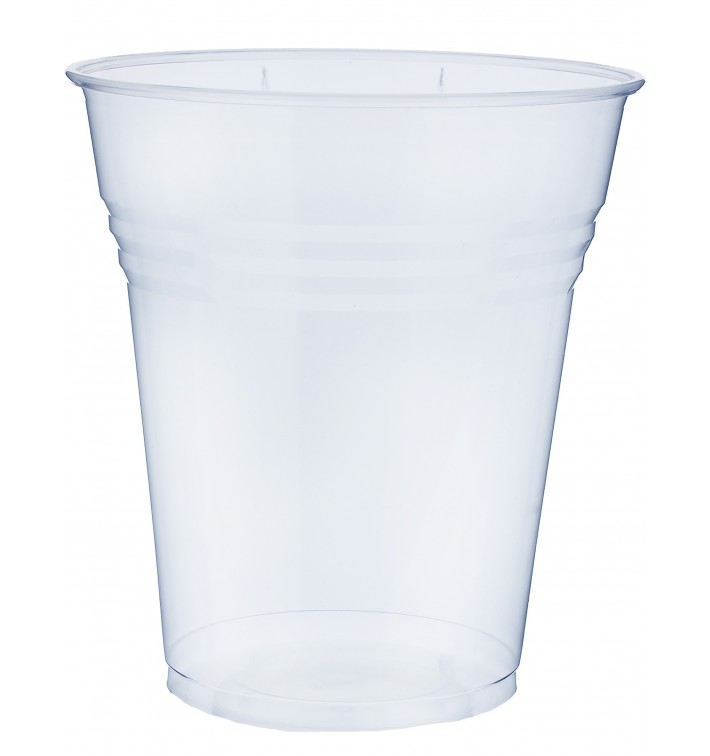
\includegraphics[width = 0.04\textwidth]{Images/transparent_cup.jpg}
\includegraphics[width = 0.07\textwidth]{Images/red_cup.jpg}};
    \node at (1.5,1.5) {};
    \node at (-1.5,-1.5) {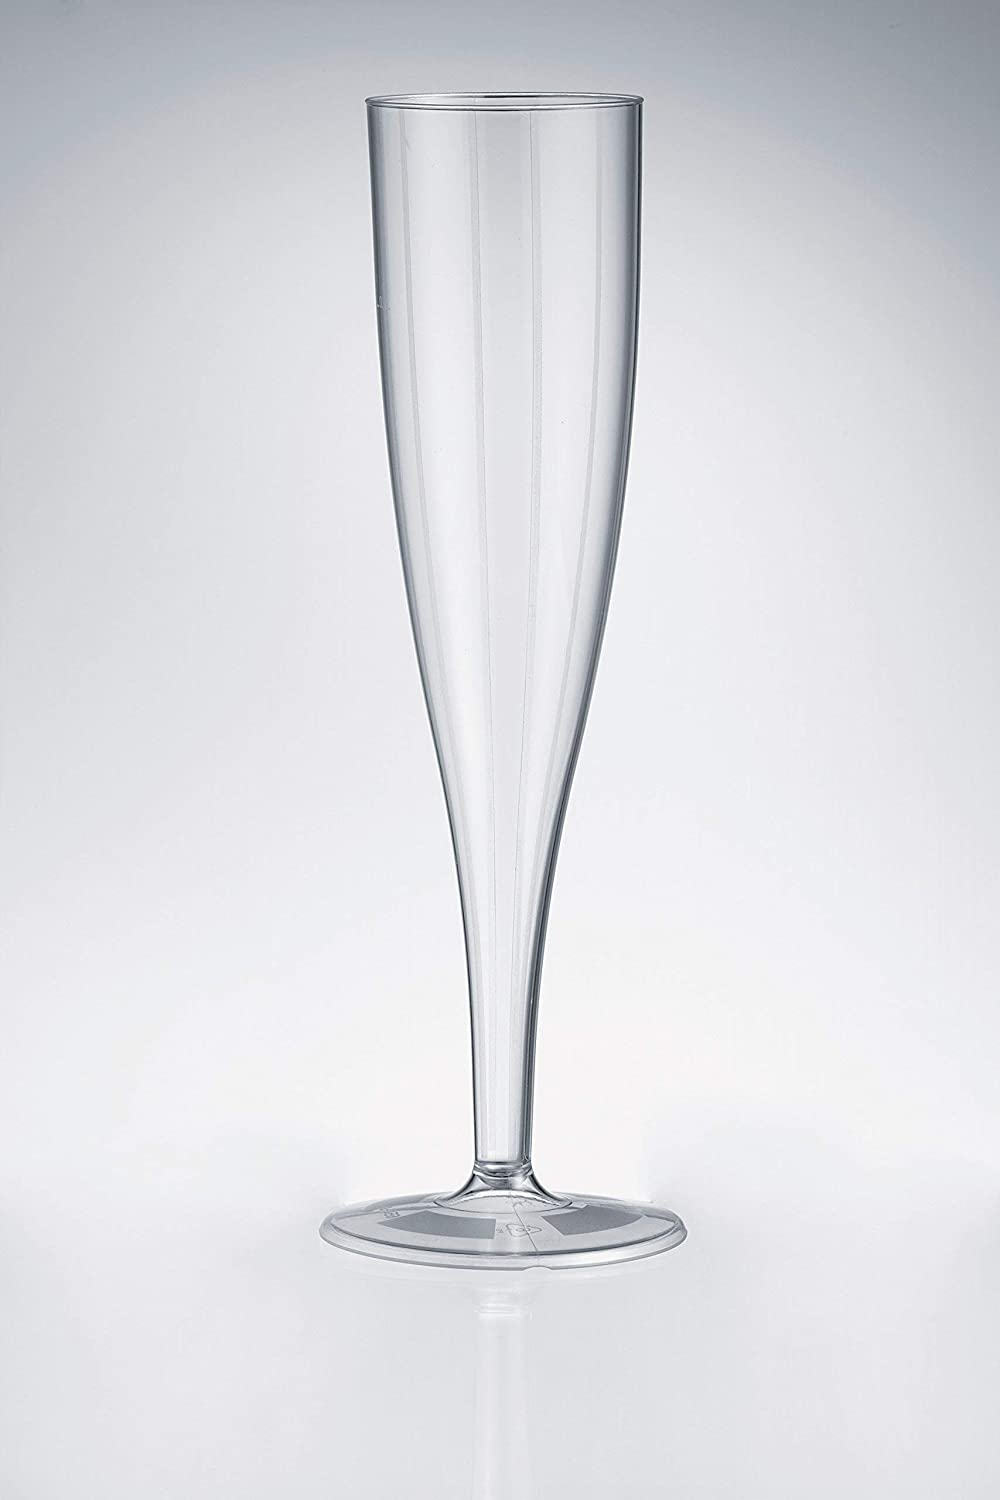
\includegraphics[width = 0.1\textwidth]{Images/champagne_cup.jpg}};
    \node at (1.5,-1.5) {
\includegraphics[width = 0.1\textwidth]{Images/wine_glass1.png}};
  \end{tikzpicture}